\documentclass[12pt,a4paper]{article}
\usepackage{fontspec}
\setmainfont{Arial}
\usepackage{polyglossia}
\setdefaultlanguage{ukrainian}
\setotherlanguage{english}
\usepackage[a4paper,margin=2.2cm]{geometry}
\usepackage{graphicx}
\usepackage{booktabs}
\usepackage{longtable}
\usepackage{array}
\usepackage{float}
\usepackage{hyperref}
\usepackage{xcolor}
\usepackage{listings}
\usepackage{fancyhdr}
\usepackage{titlesec}
\definecolor{navy}{HTML}{17233B}
\definecolor{blue}{HTML}{3D68ED}
\definecolor{light}{HTML}{F2F5FA}
\hypersetup{colorlinks=true,linkcolor=blue,urlcolor=blue}
\titleformat{\section}{\Large\bfseries\color{navy}}{}{0pt}{}
\titleformat{\subsection}{\large\bfseries\color{navy}}{}{0pt}{}
\pagestyle{fancy}
\fancyhf{}
\lhead{\small Sport Events Ukraine}
\rhead{\small Лабораторна робота}
\cfoot{\thepage}
\setlength{\headheight}{15pt}
\lstset{
  basicstyle=\ttfamily\small,
  backgroundcolor=\color{light},
  frame=single,
  rulecolor=\color{blue},
  breaklines=true,
  columns=fullflexible
}

\begin{document}

\begin{titlepage}
\centering
\vspace*{2.5cm}
{\color{blue}\Large ЛАБОРАТОРНА РОБОТА\par}
\vspace{0.8cm}
{\color{navy}\Huge\bfseries Система управління\\[0.2cm] спортивними подіями\par}
\vspace{1.2cm}
{\large PostgreSQL, вебпортал і .NET Repository + Unit of Work\par}
\vfill
\begin{flushleft}
\textbf{Виконавець:} Кашинський Владислав, група ТТП-32\\[0.4cm]
\textbf{Предмет:} Сучасні технології баз даних\\[0.4cm]
\textbf{Рік:} 2026
\end{flushleft}
\vfill
{\color{navy}\large Sport Events Ukraine\par}
\end{titlepage}

\section{Мета роботи}

Розробити нормалізовану реляційну модель спортивних подій України, реалізувати її у PostgreSQL та підключити до прикладного коду. Портал підтримує каталог подій, календар, реєстрації спортсменів, команди, змагання, матчі, результати та кабінет організатора.

\section{Середовище та технології}

\begin{itemize}
\item PostgreSQL 15+ і pgAdmin 4 - реляційна база даних.
\item SQL та PL/pgSQL - таблиці, функції, view, тригери та індекси.
\item .NET 8, Npgsql і Dapper - приклад доступу до БД.
\item HTML, CSS і JavaScript - клікабельний вебпортал.
\item dbdiagram.io - ER-модель у форматі DBML.
\item GitHub - версійне зберігання проєкту.
\end{itemize}

\section{Результат за вимогами}

\begin{longtable}{p{0.22\textwidth}p{0.68\textwidth}}
\toprule
\textbf{Вимога} & \textbf{Реалізація}\\
\midrule
15+ сутностей & 17 таблиць: користувачі, спорт, локації, події, категорії, профілі, команди, заявки, змагання, матчі, результати, спонсори та аудит.\\
Soft delete & Поле \texttt{deleted\_at} у сутностях, що можуть бути архівовані без фізичного видалення.\\
Історія змін & Поля \texttt{last\_modified\_at} і \texttt{last\_modified\_by}; окремий \texttt{audit\_log}.\\
SQL-об'єкти & 14 функцій, 4 view, тригери аудиту для прикладних таблиць.\\
Індекси & B-tree для статусу і дати події, GIN для пошуку за назвою, унікальні індекси для зв'язків.\\
Робота з коду & Repository + Unit of Work для подій і реєстрацій; запити виконуються через функції та view.\\
\bottomrule
\end{longtable}

\section{Модель даних}

ER-модель збережена у файлі \texttt{sports\_events\_portal.dbml} і доступна для перегляду в dbdiagram.io. Центральна сутність \texttt{sport\_event} пов'язана зі спортом, локацією, організатором і категоріями. Реєстрація спортсмена виконується через \texttt{event\_registration}, командна участь - через \texttt{event\_team\_entry}. Змагання, матчі та результати винесені в окремі сутності.

\begin{table}[H]
\centering
\small
\begin{tabular}{p{0.29\textwidth}p{0.59\textwidth}}
\toprule
\textbf{Група} & \textbf{Сутності}\\
\midrule
Довідники й доступ & \texttt{app\_user}, \texttt{sport}, \texttt{venue}\\
Події & \texttt{sport\_event}, \texttt{event\_category}, \texttt{event\_location}\\
Учасники & \texttt{athlete\_profile}, \texttt{team}, \texttt{team\_member}\\
Реєстрації & \texttt{event\_registration}, \texttt{event\_team\_entry}\\
Змагання & \texttt{competition}, \texttt{match}, \texttt{match\_participant}, \texttt{match\_result}\\
Партнери й контроль & \texttt{sponsor}, \texttt{event\_sponsor}, \texttt{audit\_log}\\
\bottomrule
\end{tabular}
\end{table}

\section{Нормалізація}

\begin{itemize}
\item 1НФ: усі поля атомарні, повторювані групи винесені у зв'язані таблиці.
\item 2НФ: залежності від складених ключів зберігаються у таблицях зв'язків, наприклад \texttt{team\_member} і \texttt{event\_team\_entry}.
\item 3НФ: спорт, локація, користувач, категорія та подія мають власні сутності, тому назви не дублюються у заявках і матчах.
\item Унікальні обмеження та зовнішні ключі запобігають дублюванню і сирітським записам.
\end{itemize}

\section{Реалізація PostgreSQL}

Файл \texttt{schema.sql} створює розширення \texttt{pgcrypto} і \texttt{pg\_trgm}, схему \texttt{sports}, таблиці, обмеження, функції, view, тригери та індекси. Файл \texttt{seed.sql} додає демонстраційні дані: 12 подій у 7 містах, 5 видів спорту, 14 локацій, 8 команд і 300 профілів спортсменів.

Тригер аудиту записує операції вставки, оновлення та видалення у \texttt{audit\_log}. Soft delete зберігає запис у БД, але прибирає його з активних view.

\begin{figure}[H]
\centering
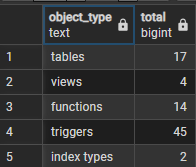
\includegraphics[width=0.74\textwidth]{screenshots/pgadmin-objects.png}
\caption{Перевірка об'єктів у pgAdmin: таблиці, view, функції, тригери та типи індексів}
\end{figure}

\section{Індекси}

Для фільтрації каталогу використано частковий B-tree індекс за \texttt{status} і \texttt{starts\_at}. Для пошуку за назвою події використано GIN індекс з триграмним розширенням. Унікальні індекси забезпечують відсутність дублювання категорій, членів команди та заявок.

Приклад перевірки плану:

\begin{lstlisting}
EXPLAIN ANALYZE
SELECT *
FROM sports.v_active_events
WHERE name ILIKE '%кубок%';
\end{lstlisting}

\section{Repository та Unit of Work}

У \texttt{repository-example.cs} реалізовано:

\begin{itemize}
\item \texttt{EventRepository} - читання подій з view та виклик функцій PostgreSQL.
\item \texttt{RegistrationRepository} - створення і скасування заявки через функції БД.
\item \texttt{EventWorkflow} - одна транзакція для створення події, категорії та публікації.
\item \texttt{UnitOfWork} - спільне підключення і транзакція для логічно пов'язаних операцій.
\end{itemize}

Такий підхід не дублює бізнес-правила у клієнті та залишає SQL-операції централізованими у базі.

\section{Вебпортал}

Вебпортал реалізований у \texttt{index.html}, \texttt{assets/app.js} і \texttt{assets/styles.css}. Перевірені сценарії:

\begin{itemize}
\item каталог з пошуком, фільтрами за видом спорту, містом і статусом;
\item таблиця та календар з переходом між місяцями;
\item деталі події з вибором однієї категорії під час реєстрації;
\item профіль учасника, історія заявок і вихід з облікового запису;
\item кабінет організатора зі списком заявок, профілями, підтвердженням і відхиленням;
\item список усіх учасників, команди і створення нової події;
\item збереження стану після оновлення сторінки через локальне сховище прототипу.
\end{itemize}

\begin{figure}[H]
\centering
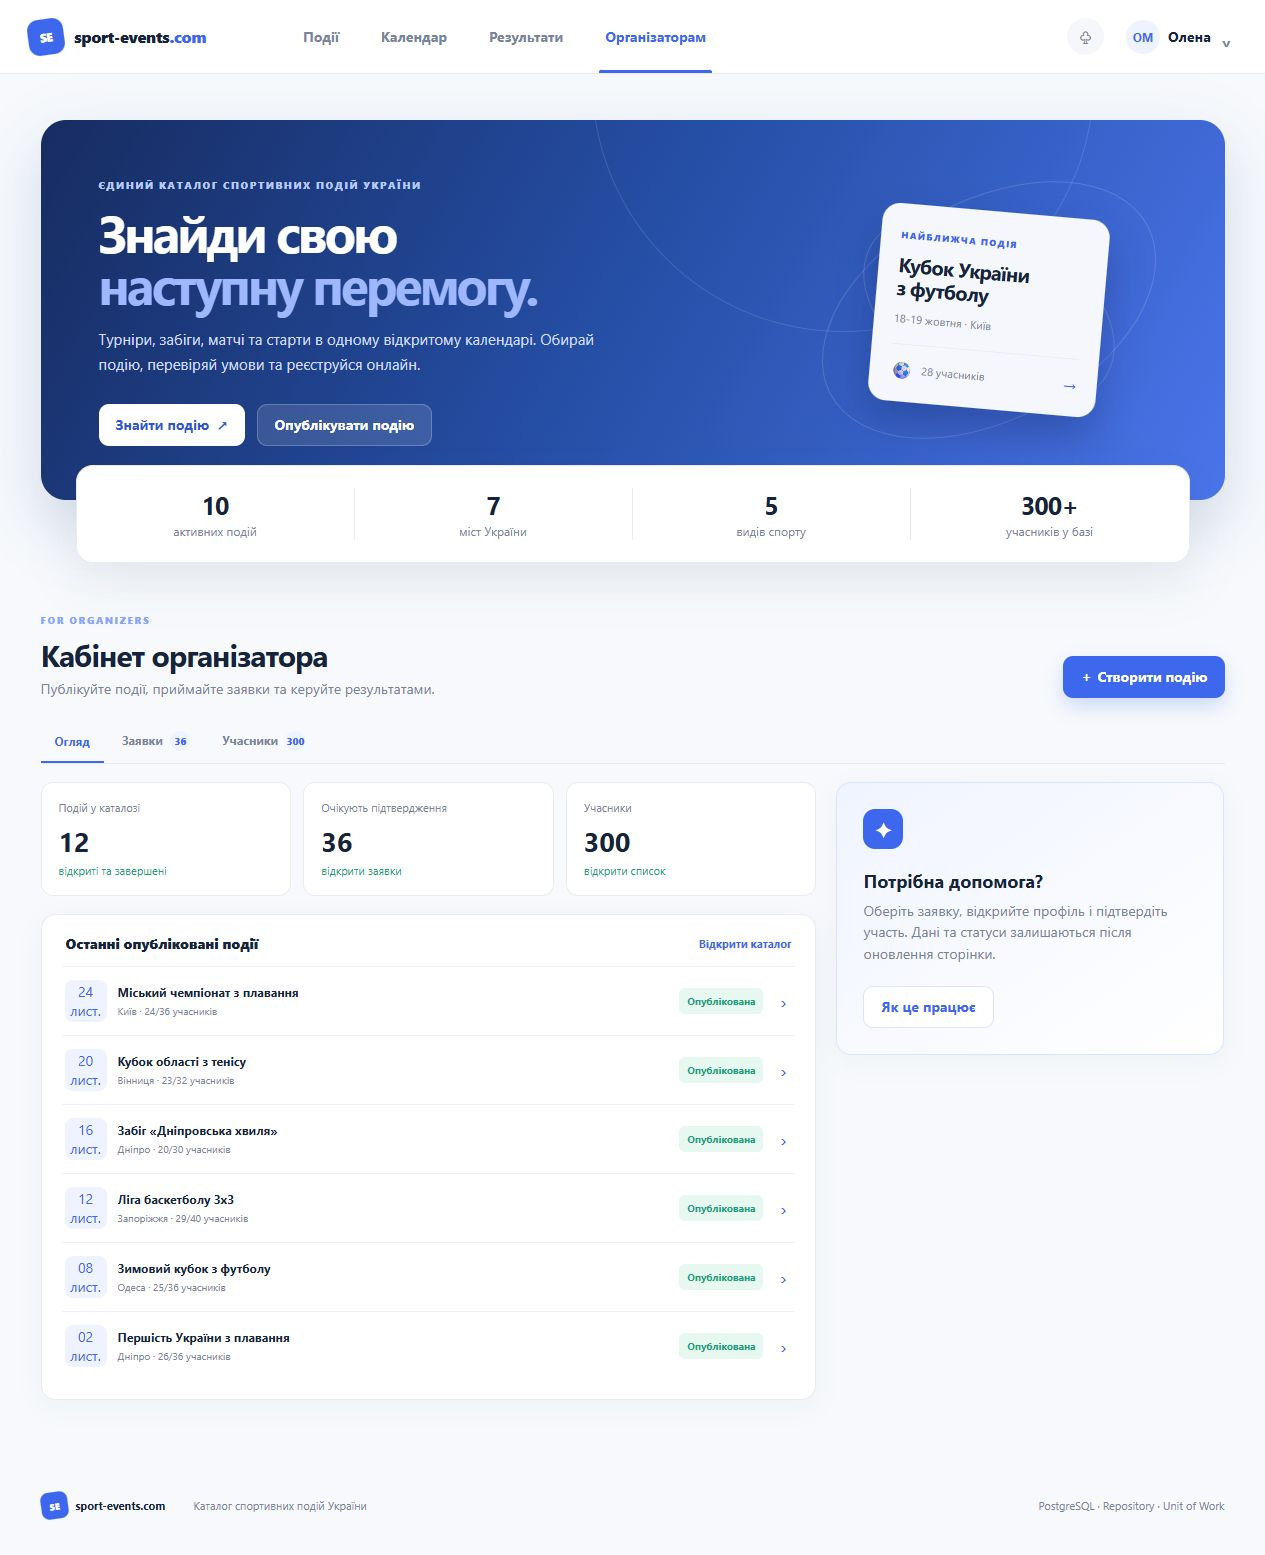
\includegraphics[width=\textwidth]{screenshots/organizer-full.png}
\caption{Актуальний кабінет організатора після виправлення верстки}
\end{figure}

\section{Перевірка}

Виконано такі перевірки:

\begin{enumerate}
\item Перевірено запуск порталу на локальному HTTP-сервері.
\item Перевірено перемикання сторінок каталогу, календаря та вкладок організатора.
\item Перевірено підтвердження заявки та оновлення лічильників.
\item Перевірено відкриття профілю учасника і списку учасників.
\item Перевірено створення події та її відновлення після оновлення сторінки.
\item Перевірено JavaScript синтаксис командою \texttt{node --check assets/app.js}.
\item Перевірено відсутність помилок у консолі браузера під час основних сценаріїв.
\end{enumerate}

\section{Висновок}

Розроблено завершений навчальний проєкт системи управління спортивними подіями. Він містить ER-модель з 17 сутностями, нормалізовану PostgreSQL-схему, SQL-функції, view, тригери, індекси, seed-дані, вебпортал та приклад Repository + Unit of Work. Усі ключові вимоги лабораторної роботи покриті окремими файлами репозиторію.

\end{document}
